\subsection*{Visitor Pattern}\label{subs:visit}
As mentioned the visitor pattern is but one way of traversing a tree.
The visitor pattern is used not only to traverse the parse tree provided by ANTLR.
The visitor pattern is implemented throughout the compiler, to both create the AST from the parse tree, for the pretty print functionality as well as filling the symbol table.
As such the visitor pattern defines the structure of the compiler, and thus understanding what is gained from using this pattern is important.
The visitor pattern is a Gang of Four, authors of ``Design Patterns: Elements of Reusable Object-Oriented Software'', design pattern.
Its description says ``The visitor pattern is a design pattern that separates a set of structured data from the functionality that may be performed upon it.''. \citep{GOF}

The pattern is a behavioural pattern i.e. it defines how communication between classes and entities are handled.
In the tree walk for the ANTLR generated parse tree, the visitor should convert the entirety into a new AST.
This entails that each different node in the parse tree must be visited and create an equivelent node for the AST.

Through use of the visitor pattern the functionality is seperated from the classes they are performed upon.
Instead the functionality is on a interface that each visitor implements.
The classes have an accept method that allows them to call the visitor in question with itself as an argument.
This allows the ability of adding new operations without changing the original data structure, an invaluable feature when doing iterative development.
\myref{image:visitor} shows a UML diagram of the visitor pattern.
This diagram is from a C# representation, and while the idea is the same the exact implementation is not identical to the one used in the compiler for GAMBLE.
The most important things to take note of are the classes ``ConcreteElement'' and ``ConcreteVisitor''.
The ``ConcreteElement'' represent the different kinds of nodes in a given tree.
The ``ConcreteVisitor'' represent the different kind of visitors implemented, this being one for AST, parse tree, symbol table, code generation and pretty print, all these implements an interface that contains visit methods for each ``ConcreteElement''.

\begin{figure}[h!]
\centering
 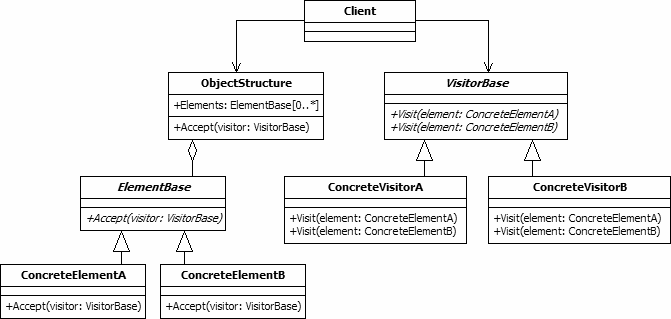
\includegraphics[width=1\textwidth]{figures/VisitorPattern.png} % trim=4.85cm 15cm 0.85cm 1cm
\caption{A UML diagram for the implementation of the visitor pattern in a C# environment}\label{image:visitor}
\vspace{-15pt}
\end{figure}




%Gang of four beskriver også denne benefit - men er ikke helt sikker på hvad den benefit rent faktisk betyder for os?
%Another benefit is that a single visitor object is used to visit all classes.
%This visitor can maintain state between calls to individual data objects. <----- dis is what im not sure of.
